\documentclass{article}

\usepackage{postprocess/context/arxiv}

\usepackage[utf8]{inputenc} % allow utf-8 input
\usepackage{amsmath}
\usepackage[T1]{fontenc}    % use 8-bit T1 fonts
\usepackage{hyperref}       % hyperlinks
\usepackage{url}            % simple URL typesetting
\usepackage{booktabs}       % professional-quality tables
\usepackage{amsfonts}       % blackboard math symbols
\usepackage{nicefrac}       % compact symbols for 1/2, etc.
\usepackage{microtype}      % microtypography
\usepackage{lipsum}		% Can be removed after putting your text content
\usepackage{graphicx}
\usepackage{natbib}
\usepackage{doi}
\usepackage{float}
\usepackage{subcaption}
\usepackage{wrapfig}

\title{Causal Discovery Report on Sachs}

\author{ \href{https://orcid.org/0000-0000-0000-0000}{
\includegraphics[scale=0.06]{postprocess/context/orcid.pdf}\hspace{1mm}Causal Copilot}}

\renewcommand{\headeright}{Technical Report}
\renewcommand{\undertitle}{Technical Report}

\hypersetup{
pdftitle={Causal Discovery Report on Sachs},
pdfauthor={Causal Copilot},
pdfkeywords={Causal Discovery, Large Language Model, PC, Sachs},
}

\begin{document}
\maketitle

\begin{abstract}
This study analyzes a dataset encompassing various gene and protein names associated with critical signaling pathways, specifically the Mitogen-Activated Protein Kinase (MAPK) pathway. We employed a systematic causal discovery methodology that included data preprocessing, algorithm selection guided by a large language model (LLM), hyperparameter tuning, and graph refinement using Bootstrap methods and LLM suggestions. The results reveal intricate regulatory interactions among key proteins, with notable findings including the self-regulatory loop between Plcg and PIP3, and the influential roles of Erk in mediating cellular functions. Our contributions lie in successfully employing advanced computational techniques to elucidate causal relationships within complex biological networks and providing a validated causal graph that enhances our understanding of cellular signaling mechanisms, which has implications for health and disease research.
\end{abstract}

\keywords{Causal Discovery, Large Language Model, PC, Sachs}

\raggedbottom
\section{Introduction}
The dataset under investigation comprises various gene and protein names closely associated with significant signaling pathways, particularly the Mitogen-Activated Protein Kinase (MAPK) pathway. The primary variables, including Raf, Mek, Plcg, PIP2, PIP3, Erk, Akt, PKA, PKC, P38, and Jnk, play pivotal roles in cellular processes such as growth, differentiation, and apoptosis. Understanding the interactions among these proteins is crucial for elucidating the underlying mechanisms of cellular signaling and their implications in health and disease. Given the complex regulatory networks and potential feedback loops among these variables, this analysis aims to uncover probable causal relationships, leveraging the known biology of these signaling cascades to inform and guide the exploratory causal discovery process.

\section{Background Knowledge}
\subsection{Detailed Explanation about the Variables}
\begin{itemize}
    \item \textbf{Raf}: Raf is a family of protein kinases that serve as key regulators in the transduction of signals for cell growth and differentiation. Activated by RAS proteins, Raf plays a pivotal role in phosphorylating MEK, thereby initiating downstream signaling cascades critical for cellular responses.
    
    \item \textbf{Mek}: Mitogen-activated protein/extracellular signal-regulated kinase kinase (MEK) acts as a dual-specificity kinase that is essential for the activation of extracellular signal-regulated kinase (Erk) through phosphorylation. As a fundamental component of the MAPK pathway, MEK mediates various cellular functions, including proliferation and survival.
    
    \item \textbf{Plcg}: Phospholipase C gamma (Plcg) is an enzyme integral to numerous cellular signaling processes, notably in generating second messengers when activated by receptor interactions. Through its catalytic function, Plcg influences various downstream signaling pathways, making it a key player in regulating cellular responses.
    
    \item \textbf{PIP2}: Phosphatidylinositol 4,5-bisphosphate (PIP2) acts as a substrate for phospholipase C, whereby it is converted into diacylglycerol (DAG) and inositol triphosphate (IP3). This phospholipid is crucial for initiating signaling cascades that regulate diverse cellular processes via second messengers.
    
    \item \textbf{PIP3}: Phosphatidylinositol 3,4,5-trisphosphate (PIP3) functions as a second messenger within the phosphoinositide 3-kinase (PI3K) signaling pathway. It plays a vital role in activating Akt and modulating various pathways involved in cell growth, metabolism, and survival.
    
    \item \textbf{Erk}: Extracellular signal-regulated kinases (Erk) are part of the MAPK signaling pathway and are involved in mediating many essential cellular processes such as differentiation, proliferation, and cellular survival. Erk activation has broad implications for the cellular response to external stimuli.
    
    \item \textbf{Akt}: Also known as Protein Kinase B, Akt is a serine/threonine kinase central to various cellular signaling pathways that promote survival, growth, and metabolism. Often activated by PIP3, Akt plays a significant role in regulating cell fate decisions.
    
    \item \textbf{PKA}: Protein kinase A (PKA) is a serine/threonine kinase activated by cyclic AMP (cAMP). This kinase regulates multiple cellular functions, including metabolism, gene expression, and cell cycle control, making it a significant player in cellular signaling dynamics.
    
    \item \textbf{PKC}: Protein kinase C (PKC) represents a family of serine/threonine kinases that are activated by diacylglycerol (DAG) and calcium ions. These kinases are involved in diverse cellular processes, including cell growth, differentiation, and apoptosis, thus highlighting their key role in cellular signaling.
    
    \item \textbf{P38}: P38 MAPK is classified as a stress-activated protein kinase, playing a crucial role in cellular responses to cytokines and stress stimuli. It is involved in various functions, including inflammation, apoptosis, and differentiation, underlining its importance in cellular stress responses.
    
    \item \textbf{Jnk}: c-Jun N-terminal kinase (Jnk), a member of the MAPK family, is activated through stress and inflammatory signals. Jnk plays significant roles in apoptosis, as well as regulating gene expression, thereby influencing multiple cellular outcomes tied to stress responses.
\end{itemize}

\subsection{Possible Causal Relations among these Variables}

\begin{minipage}[t]{0.7\linewidth}
\begin{itemize}
\item \textbf{Raf $\rightarrow$ Mek}: Raf activates Mek through phosphorylation, initiating the MAPK signaling cascade.

\item \textbf{Mek $\rightarrow$ Erk}: Mek activates Erk by phosphorylation as part of the MAPK signaling pathway.

\item \textbf{Plcg $\rightarrow$ PIP2}: Plcg hydrolyzes PIP2 to produce second messengers, playing a key role in receptor-mediated signaling.

\item \textbf{PIP2 $\rightarrow$ DAG}: PIP2 is converted to diacylglycerol (DAG) upon activation by Plcg.

\item \textbf{PIP2 $\rightarrow$ IP3}: PIP2 is cleaved by Plcg to generate inositol triphosphate (IP3), which is involved in calcium signaling.

\item \textbf{DAG $\rightarrow$ PKC}: DAG activates protein kinase C (PKC), which mediates various signaling pathways.

\item \textbf{PIP3 $\rightarrow$ Akt}: PIP3 acts as a second messenger to recruit and activate Akt, promoting cell survival and growth.

\item \textbf{Erk $\rightarrow$ P38}: Erk can activate signaling pathways that lead to the activation of P38 in response to stress signals.

\item \textbf{Stress signals $\rightarrow$ Jnk}: Stress stimuli activate Jnk, which is involved in stress response and apoptosis.

\item \textbf{PKA $\rightarrow$ Various targets}: PKA, activated by cAMP, phosphorylates various proteins, influencing multiple signaling pathways and cellular processes.
\end{itemize}
\end{minipage}
\hspace{0.05\textwidth}
\begin{minipage}[t]{0.3\linewidth}
\begin{figure}[H]
\centering
\resizebox{\linewidth}{!}{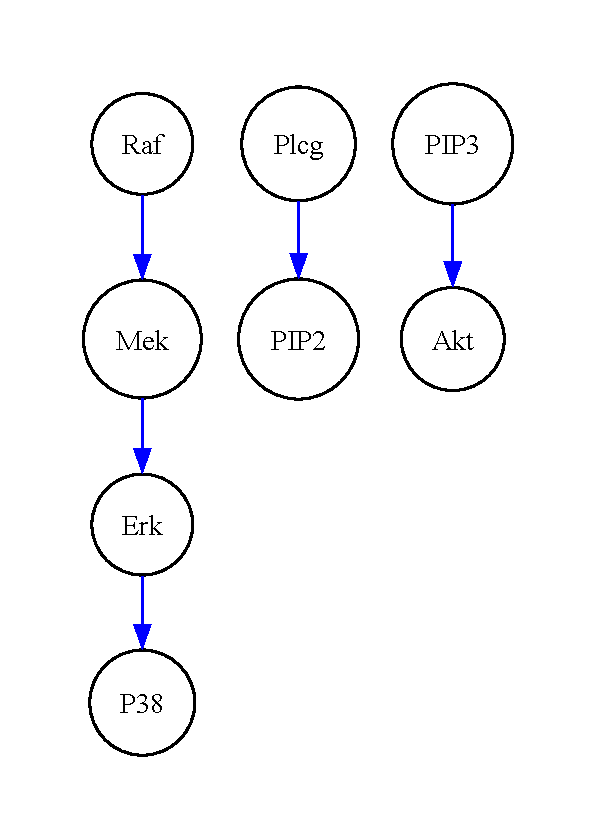
\includegraphics[height=0.3\textheight]{./demo_data/20241104_135804/sachs/output_graph/potential_relation.pdf}}
\caption{\label{fig:relation}Possible Causal Relation Graph}
\end{figure}
\end{minipage}

\section{Dataset Descriptions and EDA}
The following is a preview of our original dataset.

\begin{table}[H]
    \centering
    \caption{Dataset Preview}
    
    \resizebox{\textwidth}{!}{
                \begin{tabular}{rrrrrrrrrrr}
\toprule
 Raf &  Mek &  Plcg &  PIP2 &  PIP3 &   Erk &  Akt &   PKA &   PKC &  P38 &  Jnk \\
\midrule
26.4 & 13.2 &  8.82 & 18.30 & 58.80 &  6.61 & 17.0 & 414.0 & 17.00 & 44.9 & 40.0 \\
35.9 & 16.5 & 12.30 & 16.80 &  8.13 & 18.60 & 32.5 & 352.0 &  3.37 & 16.5 & 61.5 \\
59.4 & 44.1 & 14.60 & 10.20 & 13.00 & 14.90 & 32.5 & 403.0 & 11.40 & 31.9 & 19.5 \\
73.0 & 82.8 & 23.10 & 13.50 &  1.29 &  5.83 & 11.8 & 528.0 & 13.70 & 28.6 & 23.1 \\
33.7 & 19.8 &  5.19 &  9.73 & 24.80 & 21.10 & 46.1 & 305.0 &  4.66 & 25.7 & 81.3 \\
\bottomrule
\end{tabular}
                }
                
\end{table}

\subsection{Data Properties}
We employ several statistical methods to identify data properties.

The shape of the data, data types, and missing values are assessed directly from the dataframe.
Linearity is evaluated using Ramsey’s RESET test, followed by the Benjamini \& Yekutieli procedure for multiple test correction.
Gaussian noise is assessed through the Shapiro-Wilk test, also applying the Benjamini \& Yekutieli procedure for multiple test correction.
Time-Series and Heterogeneity are derived from user queries.

Properties of the dataset we analyzed are listed below.

\begin{table}[H]
    \centering
    \caption{Data Properties}

        \begin{tabular}{rrrrrrr}
        \toprule
        Shape ($n$ x $d$) & Data Type & Missing Value & Linearity & Gaussian Errors & Time-Series & Heterogeneity \\
        \midrule
        (853, 11)   & Continuous & False & False & False & False & False \\
        \bottomrule
        \end{tabular}
        
\end{table}


\subsection{Distribution Analysis}
The following figure shows distributions of different variables. The orange dash line represents the mean, 
and the black line represents the median. Variables are categorized into three types according to their distribution characteristics.

\begin{figure}[H]
\centering
\includegraphics[width=\linewidth]{./demo_data/20241104_135804/sachs/output_graph/eda_dist.jpg}
\caption{\label{fig:dist}Distribution Plots of Variables}
\end{figure}

\begin{itemize}
\item Slight left skew distributed variables: None
\item Slight right skew distributed variables: Raf, Mek, Plcg, PIP2, PIP3, Erk, Akt, PKA, PKC, P38, Jnk
\item Symmetric distributed variables: None
\end{itemize}

\subsection{Correlation Analysis}

\begin{minipage}[t]{0.5\linewidth}
    In this analysis, we will categorize the correlation statistics of features in the dataset into three distinct categories: Strong correlations, Moderate correlations, and Weak correlations.

\begin{itemize}
\item Strong Correlated Variables: Akt and Erk
\item Moderate Correlated Variables: Mek and Raf, P38 and PKC
\item Weak Correlated Variables: None
\end{itemize}
\vfill
\end{minipage}
\hfill
\begin{minipage}[t]{0.5\linewidth}
    \begin{figure}[H]
        \centering
        \vspace{-1.5cm}
        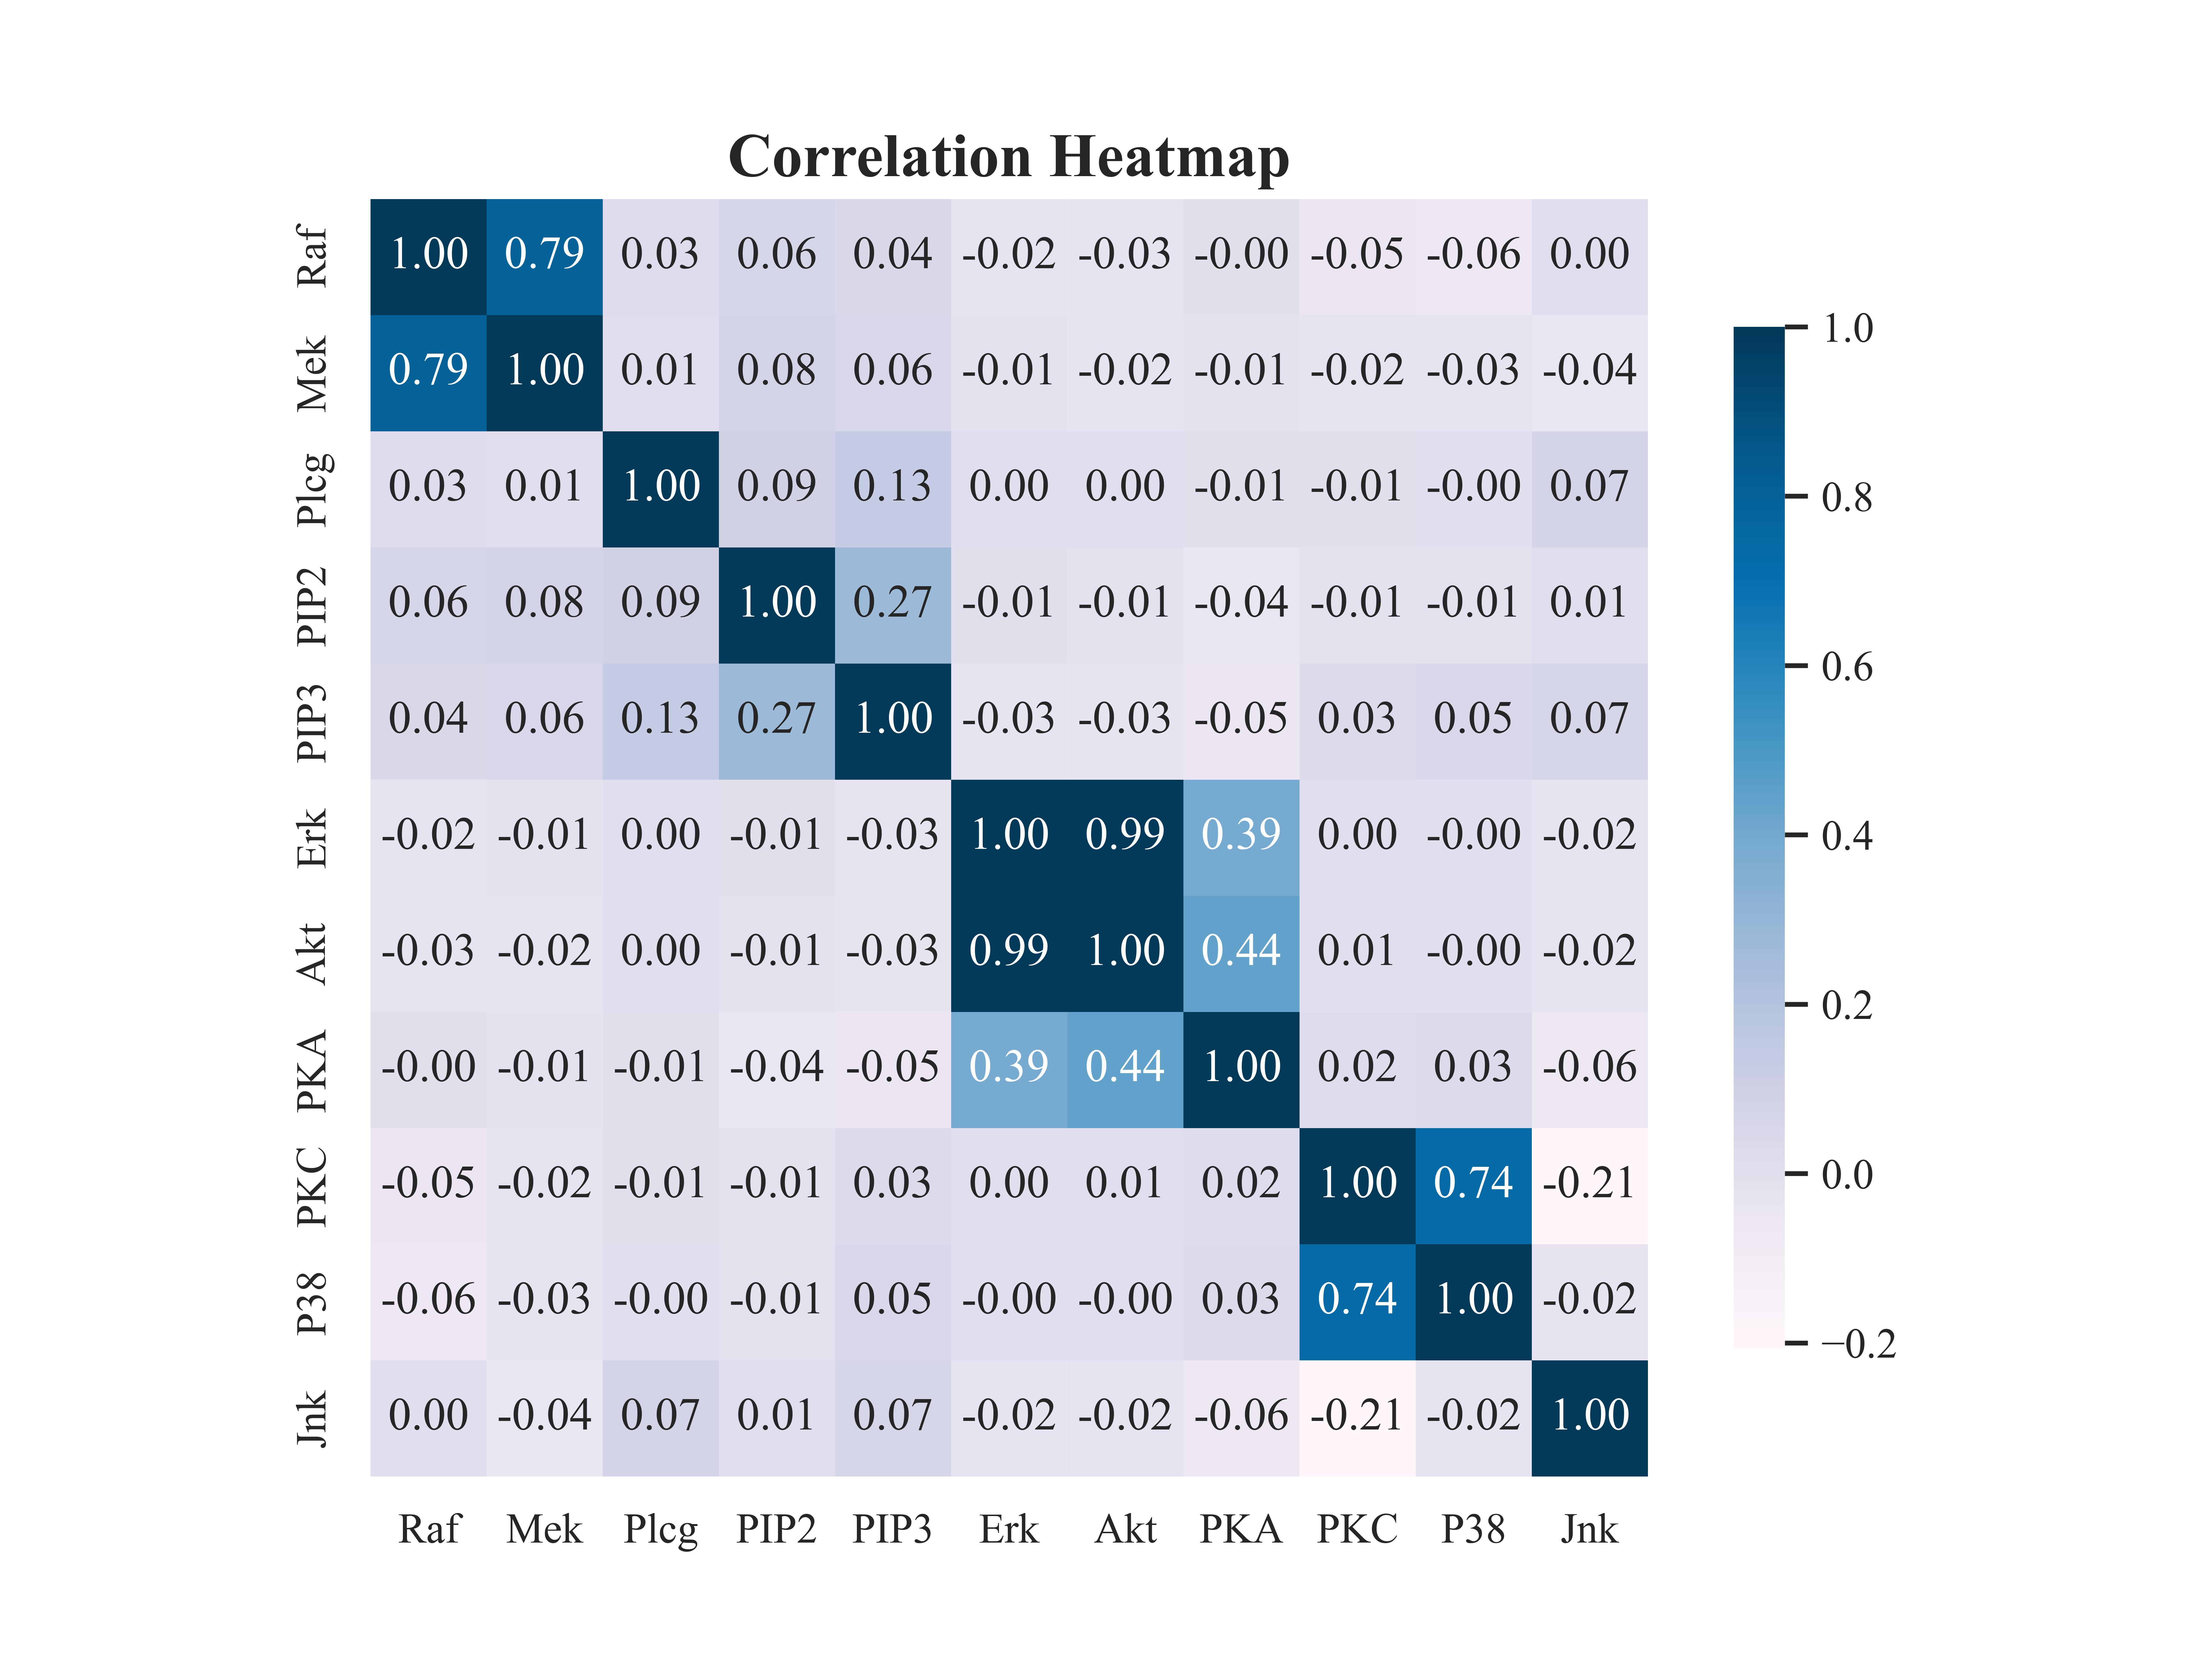
\includegraphics[width=\linewidth]{./demo_data/20241104_135804/sachs/output_graph/eda_corr.jpg}
        \caption{\label{fig:corr}Correlation Heatmap of Variables}
    \end{figure}
\end{minipage}

\section{Discovery Procedure}

In this section, we provide a detailed description of the causal discovery process implemented by Causal Copilot. 
We also provide the chosen algorithms and hyperparameters, along with the justifications for these selections.

\subsection{Data Preprocessing}
In this initial step, we preprocessed the data and examined its statistical characteristics. 
This involved cleaning the data, handling missing values, and performing exploratory data analysis to understand distributions and relationships between variables.
                
\subsection{Algorithm Selection assisted with LLM}
Following data preprocessing, we employed a large language model (LLM) to assist in 
selecting appropriate algorithms for causal discovery based on the statistical characteristics of the dataset and relevant background knowledge. 
The top three chosen algorithms, listed in order of suitability, are as follows:   

\begin{itemize}

\item \textbf{PC}:
\begin{itemize}
    \item \textbf{Description}: The PC algorithm is a constraint-based method that learns the structure of a causal graph from data by testing conditional independencies between variables. It constructs a directed acyclic graph (DAG) representing the causal relationships.
    \item \textbf{Justification}: Given that the dataset is large and with no missing values, PC is efficient for large-scale datasets and can quickly prune unnecessary edges, making it highly suitable for the described dataset.
\end{itemize}

\item \textbf{GES}:
\begin{itemize}
    \item \textbf{Description}: Greedy Equivalence Search (GES) is a score-based causal discovery algorithm that identifies the optimal causal structure by navigating the space of equivalence classes of Directed Acyclic Graphs (DAGs).
    \item \textbf{Justification}: The GES algorithm offers the ability to handle large datasets, and since the relationships are non-linear, it could still perform well using a generalized score. It effectively balances computational efficiency with the need for a comprehensive search.
\end{itemize}

\item \textbf{NOTEARS}:
\begin{itemize}
    \item \textbf{Description}: NOTEARS transforms the combinatorial problem of learning Directed Acyclic Graphs (DAGs) into a continuous optimization problem. It is particularly suited for high-dimensional data.
    \item \textbf{Justification}: Since the dataset is not highly heterogeneous and consists of continuous variables, NOTEARS is suitable for discovering causal relationships under the assumption of linearity and can leverage its optimization method effectively in this context.
\end{itemize}

\end{itemize}
                    

\subsection{Hyperparameter Values Proposal assisted with LLM}
Once the algorithms were selected, the LLM aided in proposing hyperparameters 
for the chosen algorithm, which are specified below:
        
\begin{itemize}

\item \textbf{alpha}:
\begin{itemize}
    \item \textbf{Value}: 0.05
    \item \textbf{Explanation}: Given the sample size of 853, which is within the range (500-10000), an alpha level of 0.05 is appropriate. This value balances the risk of Type I errors while maintaining reliability in detecting causal relationships in the dataset.
\end{itemize}

\item \textbf{indep\_test}:
\begin{itemize}
    \item \textbf{Value}: fisherz
    \item \textbf{Explanation}: Despite the non-Gaussian nature of the data and non-linearity, the PC algorithm's choice of Fisher's Z test is still the default for continuous data. Alternative independence tests can be explored to address violations of assumptions, but Fisher's Z remains the standard choice for initial assessments.
\end{itemize}

\item \textbf{depth}:
\begin{itemize}
    \item \textbf{Value}: -1
    \item \textbf{Explanation}: With 11 features, the graph is not very large, and allowing unlimited depth (-1) will facilitate a more thorough exploration of potential causal relationships without imposing unnecessary limitations on the search process.
\end{itemize}

\end{itemize}
                    

\subsection{Graph Tuning with Bootstrap and LLM Suggestion}
In the final step, we performed graph tuning with suggestions provided by the Bootstrap and LLM.
            
Firstly, we use the Bootstrap technique to get how much confidence we have on each edge in the initial graph.
If the confidence probability of a certain edge is greater than 95\% and it is not in the initial graph, we force it.
Otherwise, if the confidence probability is smaller than 5\% and it exists in the initial graph, we change it to the edge type with the highest probability.
            
After that, we utilize LLM to help us prune edges and determine the direction of undirected edges according to its knowledge repository.
In this step LLM can use background knowledge to add some edges that are neglected by Statistical Methods.
Voting techniques are used to enhance the robustness of results given by LLM, and the results given by LLM should not change results given by Bootstrap.

By integrating insights from both of Bootstrap and LLM to refine the causal graph, we can achieve improvements in the graph's accuracy and robustness.
            

\section{Results Summary}

\subsection{Initial Graph}

\begin{figure}[H]
    \centering
    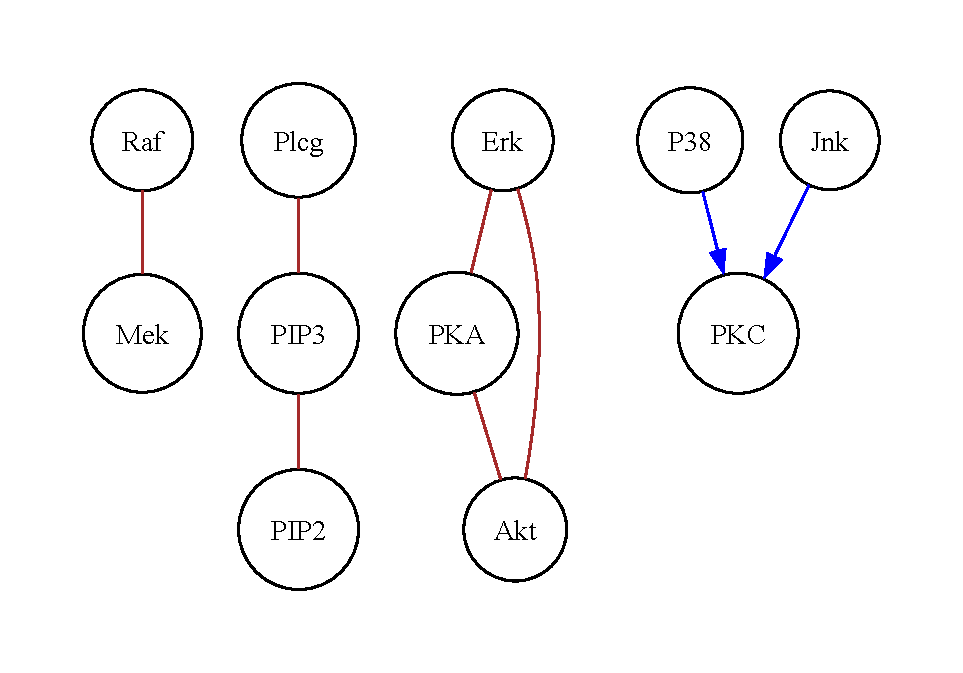
\includegraphics[height=0.3\textheight]{./demo_data/20241104_135804/sachs/output_graph/initial_graph.pdf}
    \caption{Initial Graph}
\end{figure}

The above is the initial result graph produced by our algorithm.

The analysis reveals a complex interplay among key signaling molecules, where Mek is implicated in the regulation of Raf, indicating a signaling pathway that can influence cellular responses. Plcg activates PIP3, suggesting a crucial role for this pathway in producing PIP3 which then not only stimulates the further production of PIP2 but also feeds back into the Plcg mechanism, demonstrating a self-regulatory loop. Erk emerges as a significant connector, influencing both Akt and PKA, underlining its role in mediating various cellular functions such as growth and metabolism. The bidirectional influences among Akt, Erk, and PKA suggest a feedback mechanism that enhances the robustness of signaling, allowing cells to fine-tune their responses to external stimuli. Additionally, P38 and Jnk specifically regulate PKC, indicating a distinct pathway that relates to stress responses, thus highlighting the dynamic and interconnected nature of these signaling pathways that collectively orchestrate cellular behavior.

\subsection{Revised Graph}

\begin{minipage}[t]{0.6\linewidth}
    
By using the method mentioned in Section 4.4, we provide a revised graph pruned with Bootstrap and LLM suggestion.
Pruning results are as follows.
        
Bootstrap doesn't force or forbid any edges.
            
The following are force results given by LLM:
            
\begin{itemize}
            
    \item \textbf{Raf $\rightarrow$ Erk}: Raf activates Erk through the MAPK signaling pathway by phosphorylating Mek, which in turn activates Erk, thus establishing a direct causal relationship.
                
    \item \textbf{Mek $\rightarrow$ Erk}: Mek is responsible for the phosphorylation and activation of Erk, making Mek a direct activator in the signaling cascade leading to Erk's activation.
                
    \item \textbf{Plcg $\rightarrow$ PIP2}: Plcg acts specifically on PIP2, cleaving it to generate second messengers that facilitate further signaling interactions, indicating a causal influence of Plcg on PIP2.
                
    \item \textbf{P38 $\rightarrow$ Jnk}: P38 can activate Jnk as part of the stress-activated protein kinase pathways, thereby linking P38 activation to the regulatory activity of Jnk in response to stress stimuli.
                
\end{itemize}
            
The following are directions of remaining undirected edges determined by the LLM:
\begin{itemize}

    \item \textbf{Raf $\rightarrow$ Mek}: Raf activates Mek through phosphorylation, which is a key step in the MAPK signaling pathway.

    \item \textbf{PIP2 $\rightarrow$ PIP3}: PIP2 is phosphorylated by PI3-kinase to produce PIP3, which serves as an important second messenger in cellular signaling.

    \item \textbf{Erk $\rightarrow$ Akt}: While Erk does not directly activate Akt, it plays a supportive role in the signaling pathways that can lead to Akt activation, particularly through feedback mechanisms and cross-talk within signaling networks.

\end{itemize}
            
This structured approach ensures a comprehensive and methodical analysis of the causal relationships within the dataset.
        
\vfill
\end{minipage}
\hfill
\begin{minipage}[t]{0.4\linewidth}
    \begin{figure}[H]
        \centering
        \vspace{-0.5cm}
        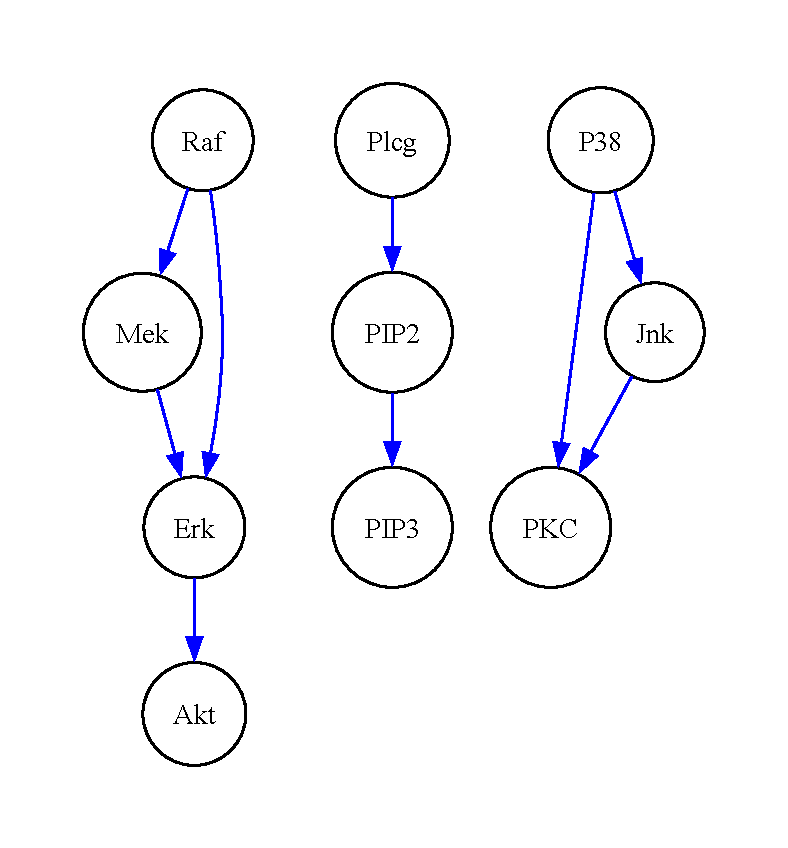
\includegraphics[width=\linewidth]{./demo_data/20241104_135804/sachs/output_graph/revised_graph.pdf}
        \caption{\label{fig:corr}Revised Graph}
    \end{figure}
\end{minipage}


\subsection{Graph Reliability Analysis}

\begin{figure}[H]
    \centering

\begin{subfigure}{0.32\textwidth}
        \centering
        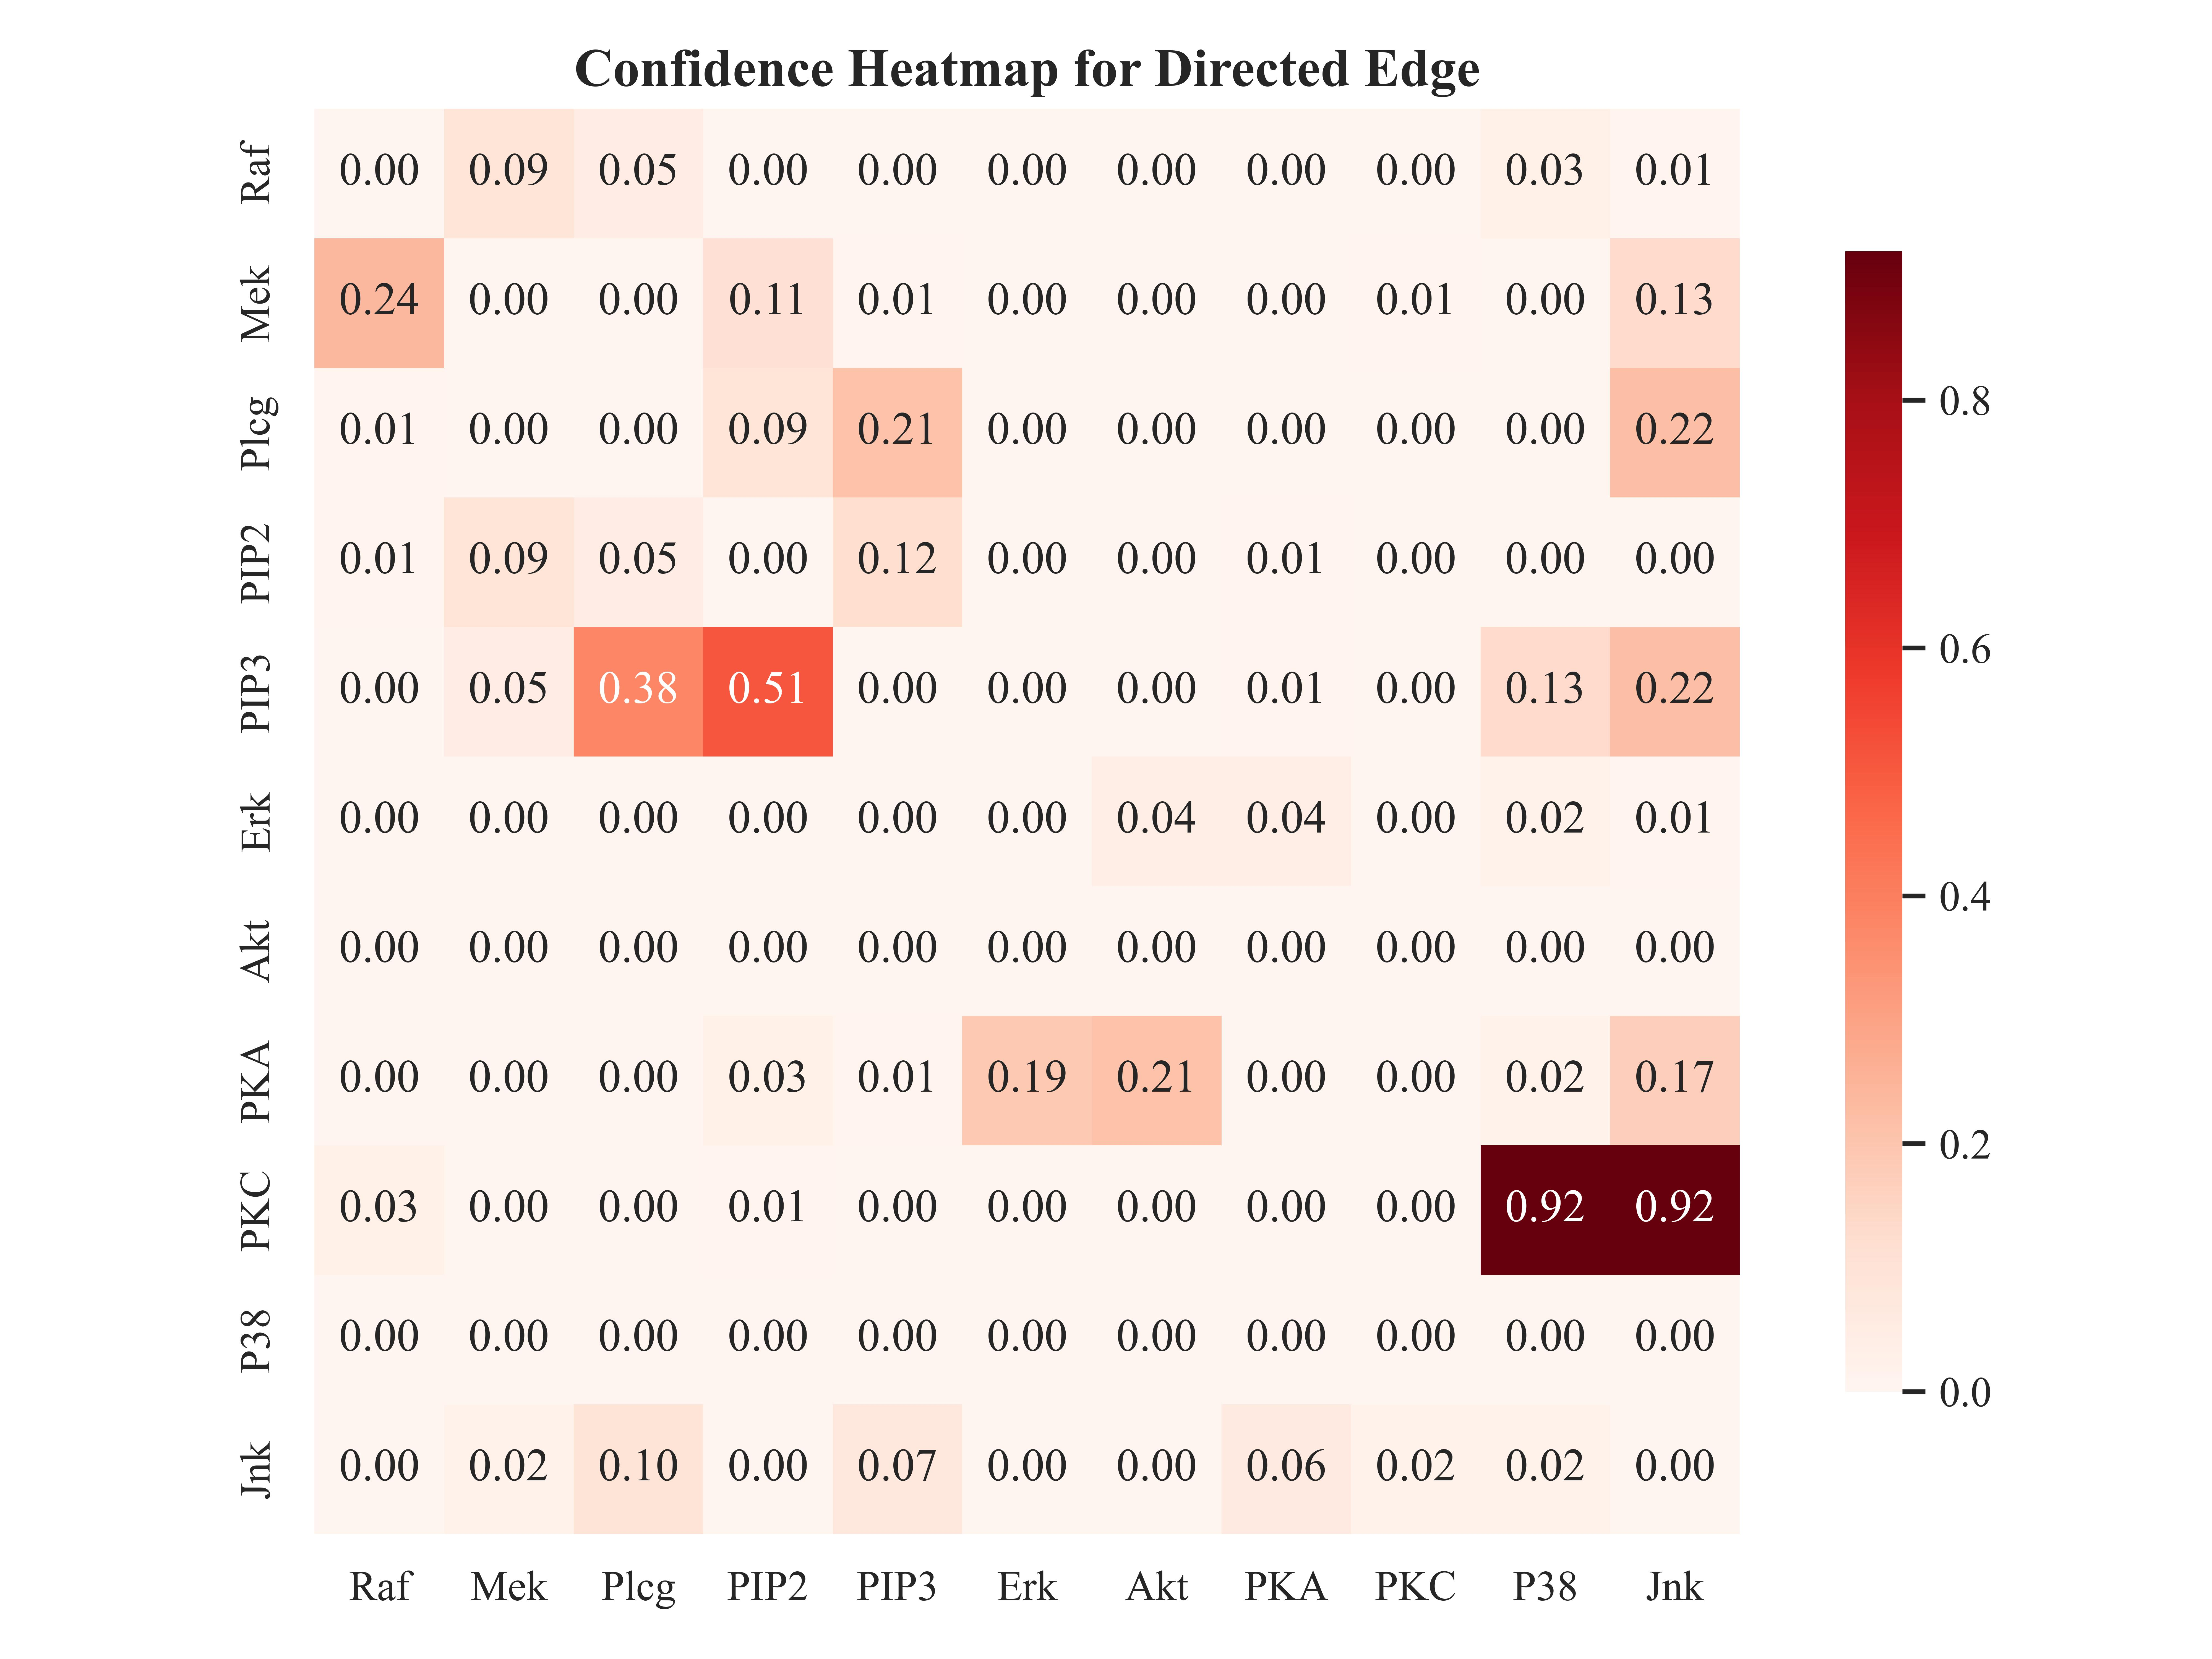
\includegraphics[width=\linewidth]{./demo_data/20241104_135804/sachs/output_graph/certain_edges_confidence_heatmap.jpg}
        \caption{Directed Edge Edge}
\end{subfigure}
\begin{subfigure}{0.32\textwidth}
        \centering
        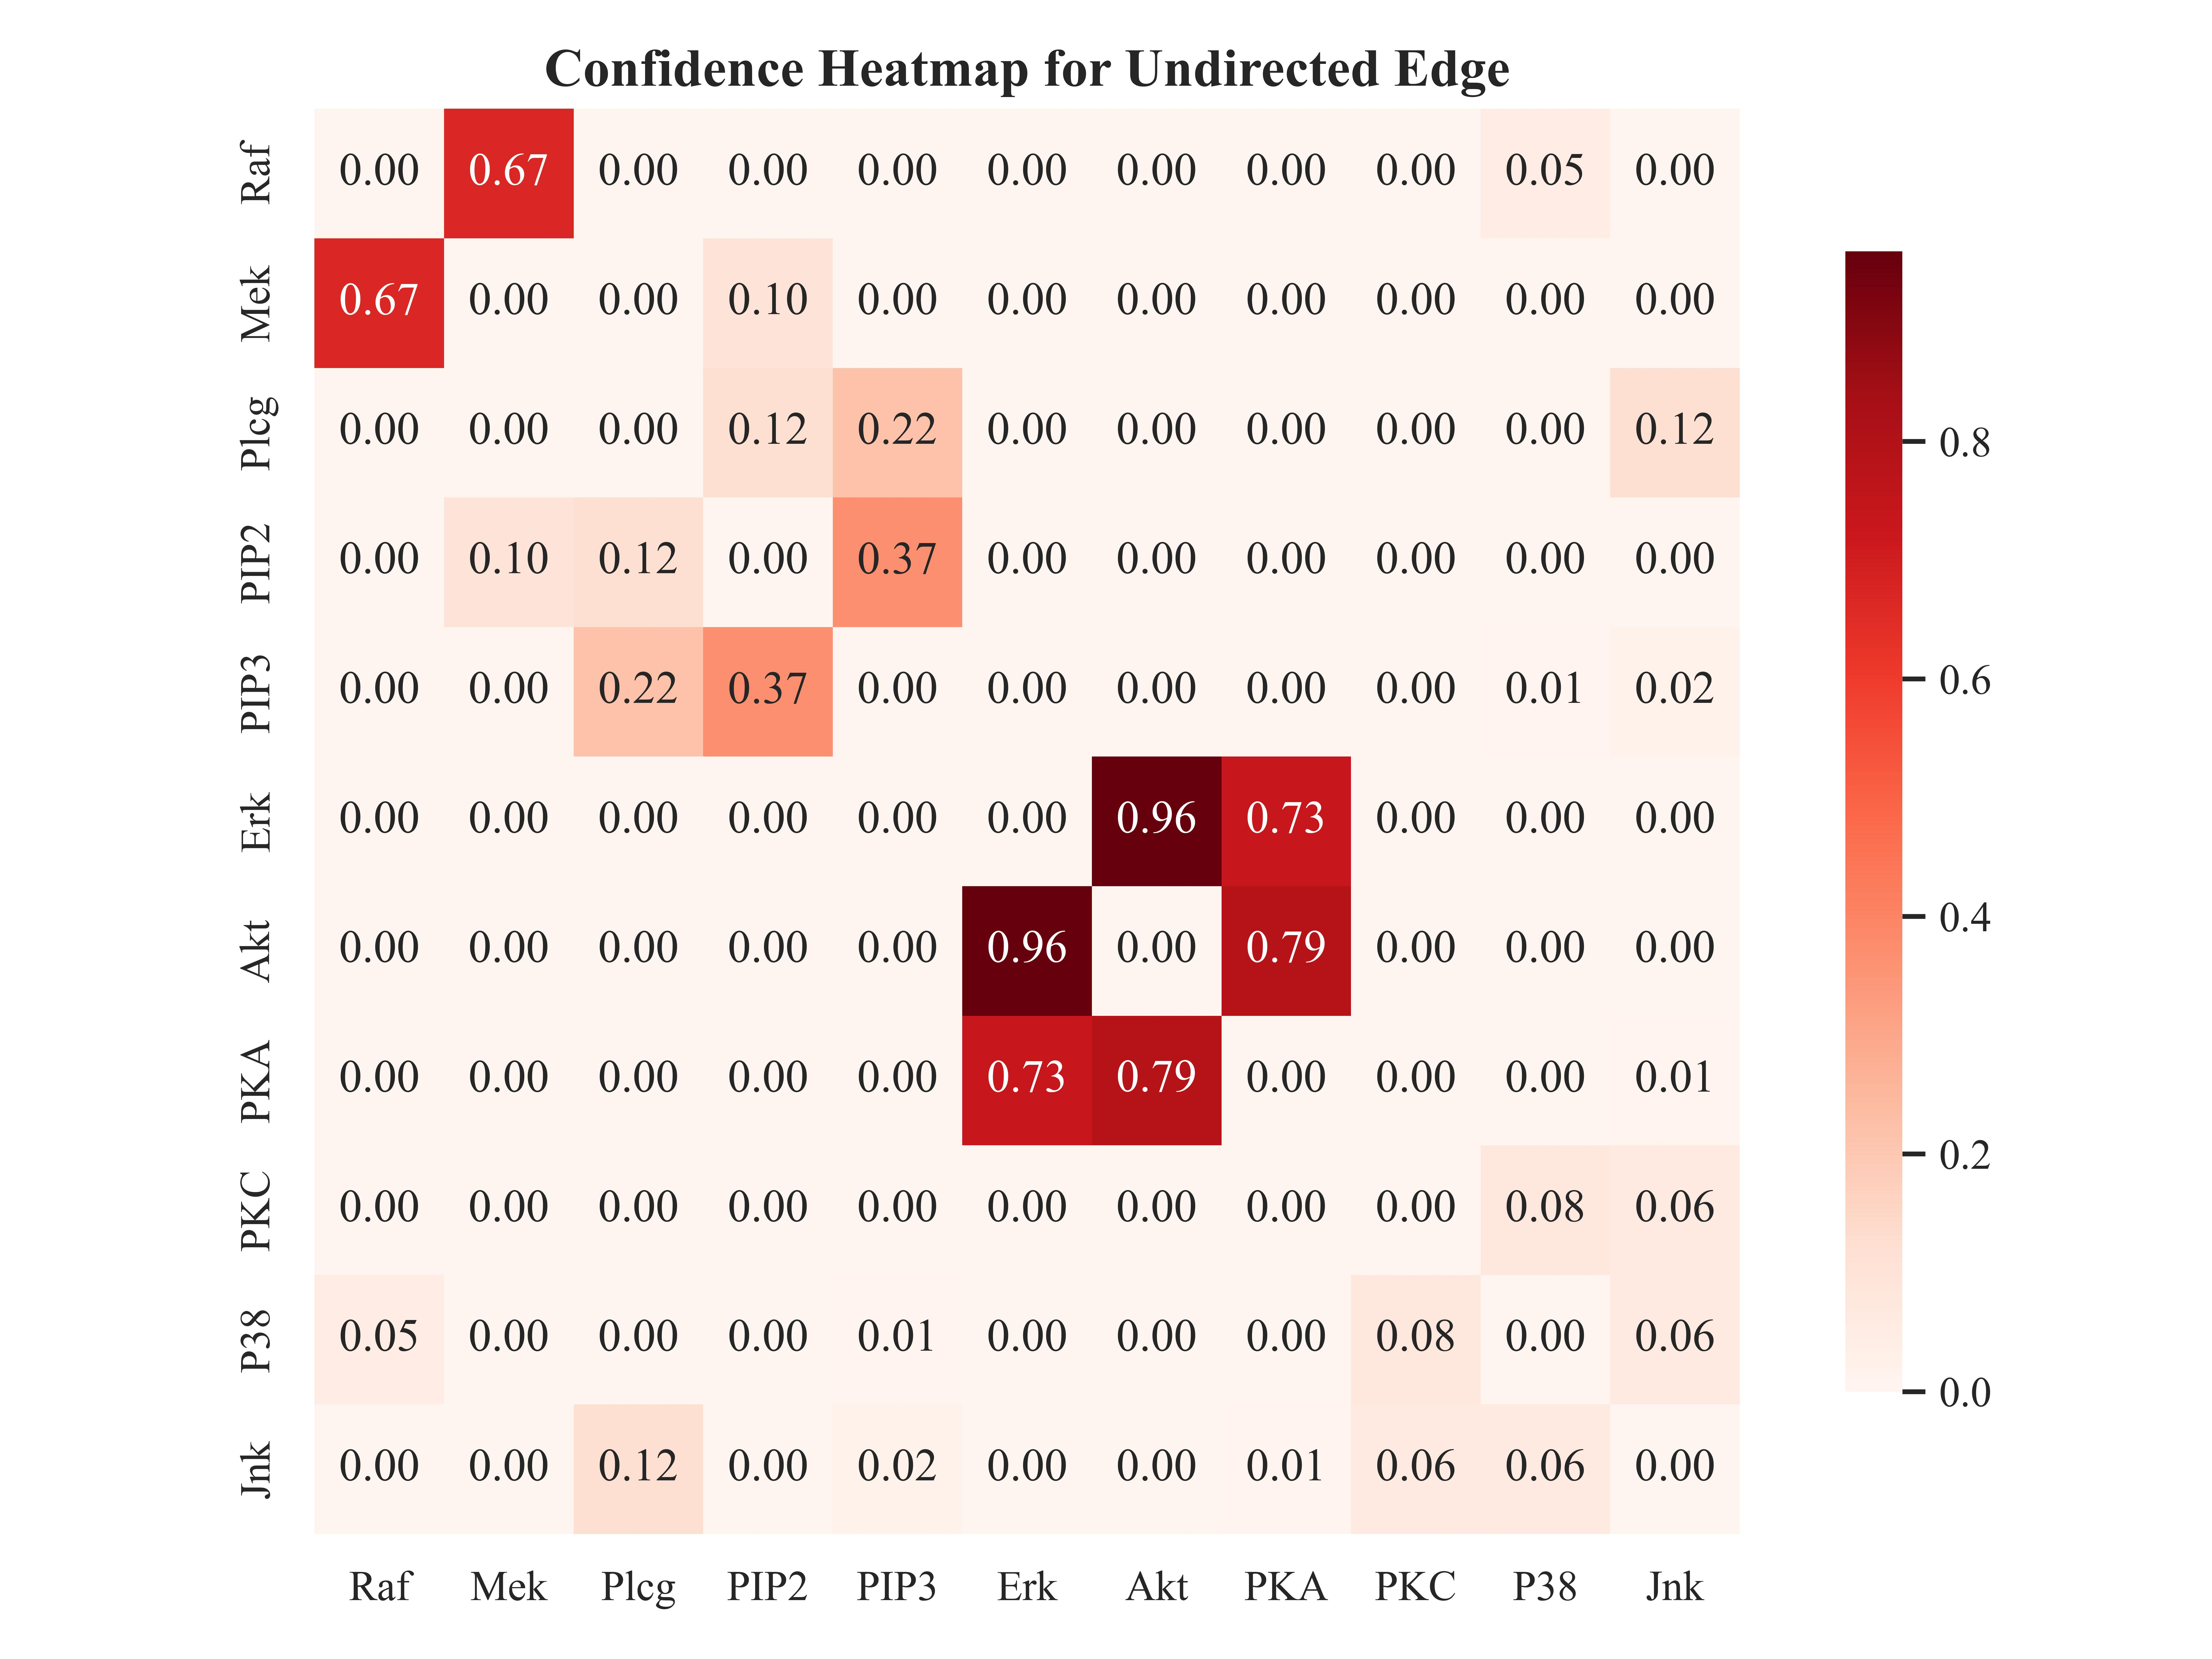
\includegraphics[width=\linewidth]{./demo_data/20241104_135804/sachs/output_graph/uncertain_edges_confidence_heatmap.jpg}
        \caption{Undirected Edge Edge}
\end{subfigure}
\begin{subfigure}{0.32\textwidth}
        \centering
        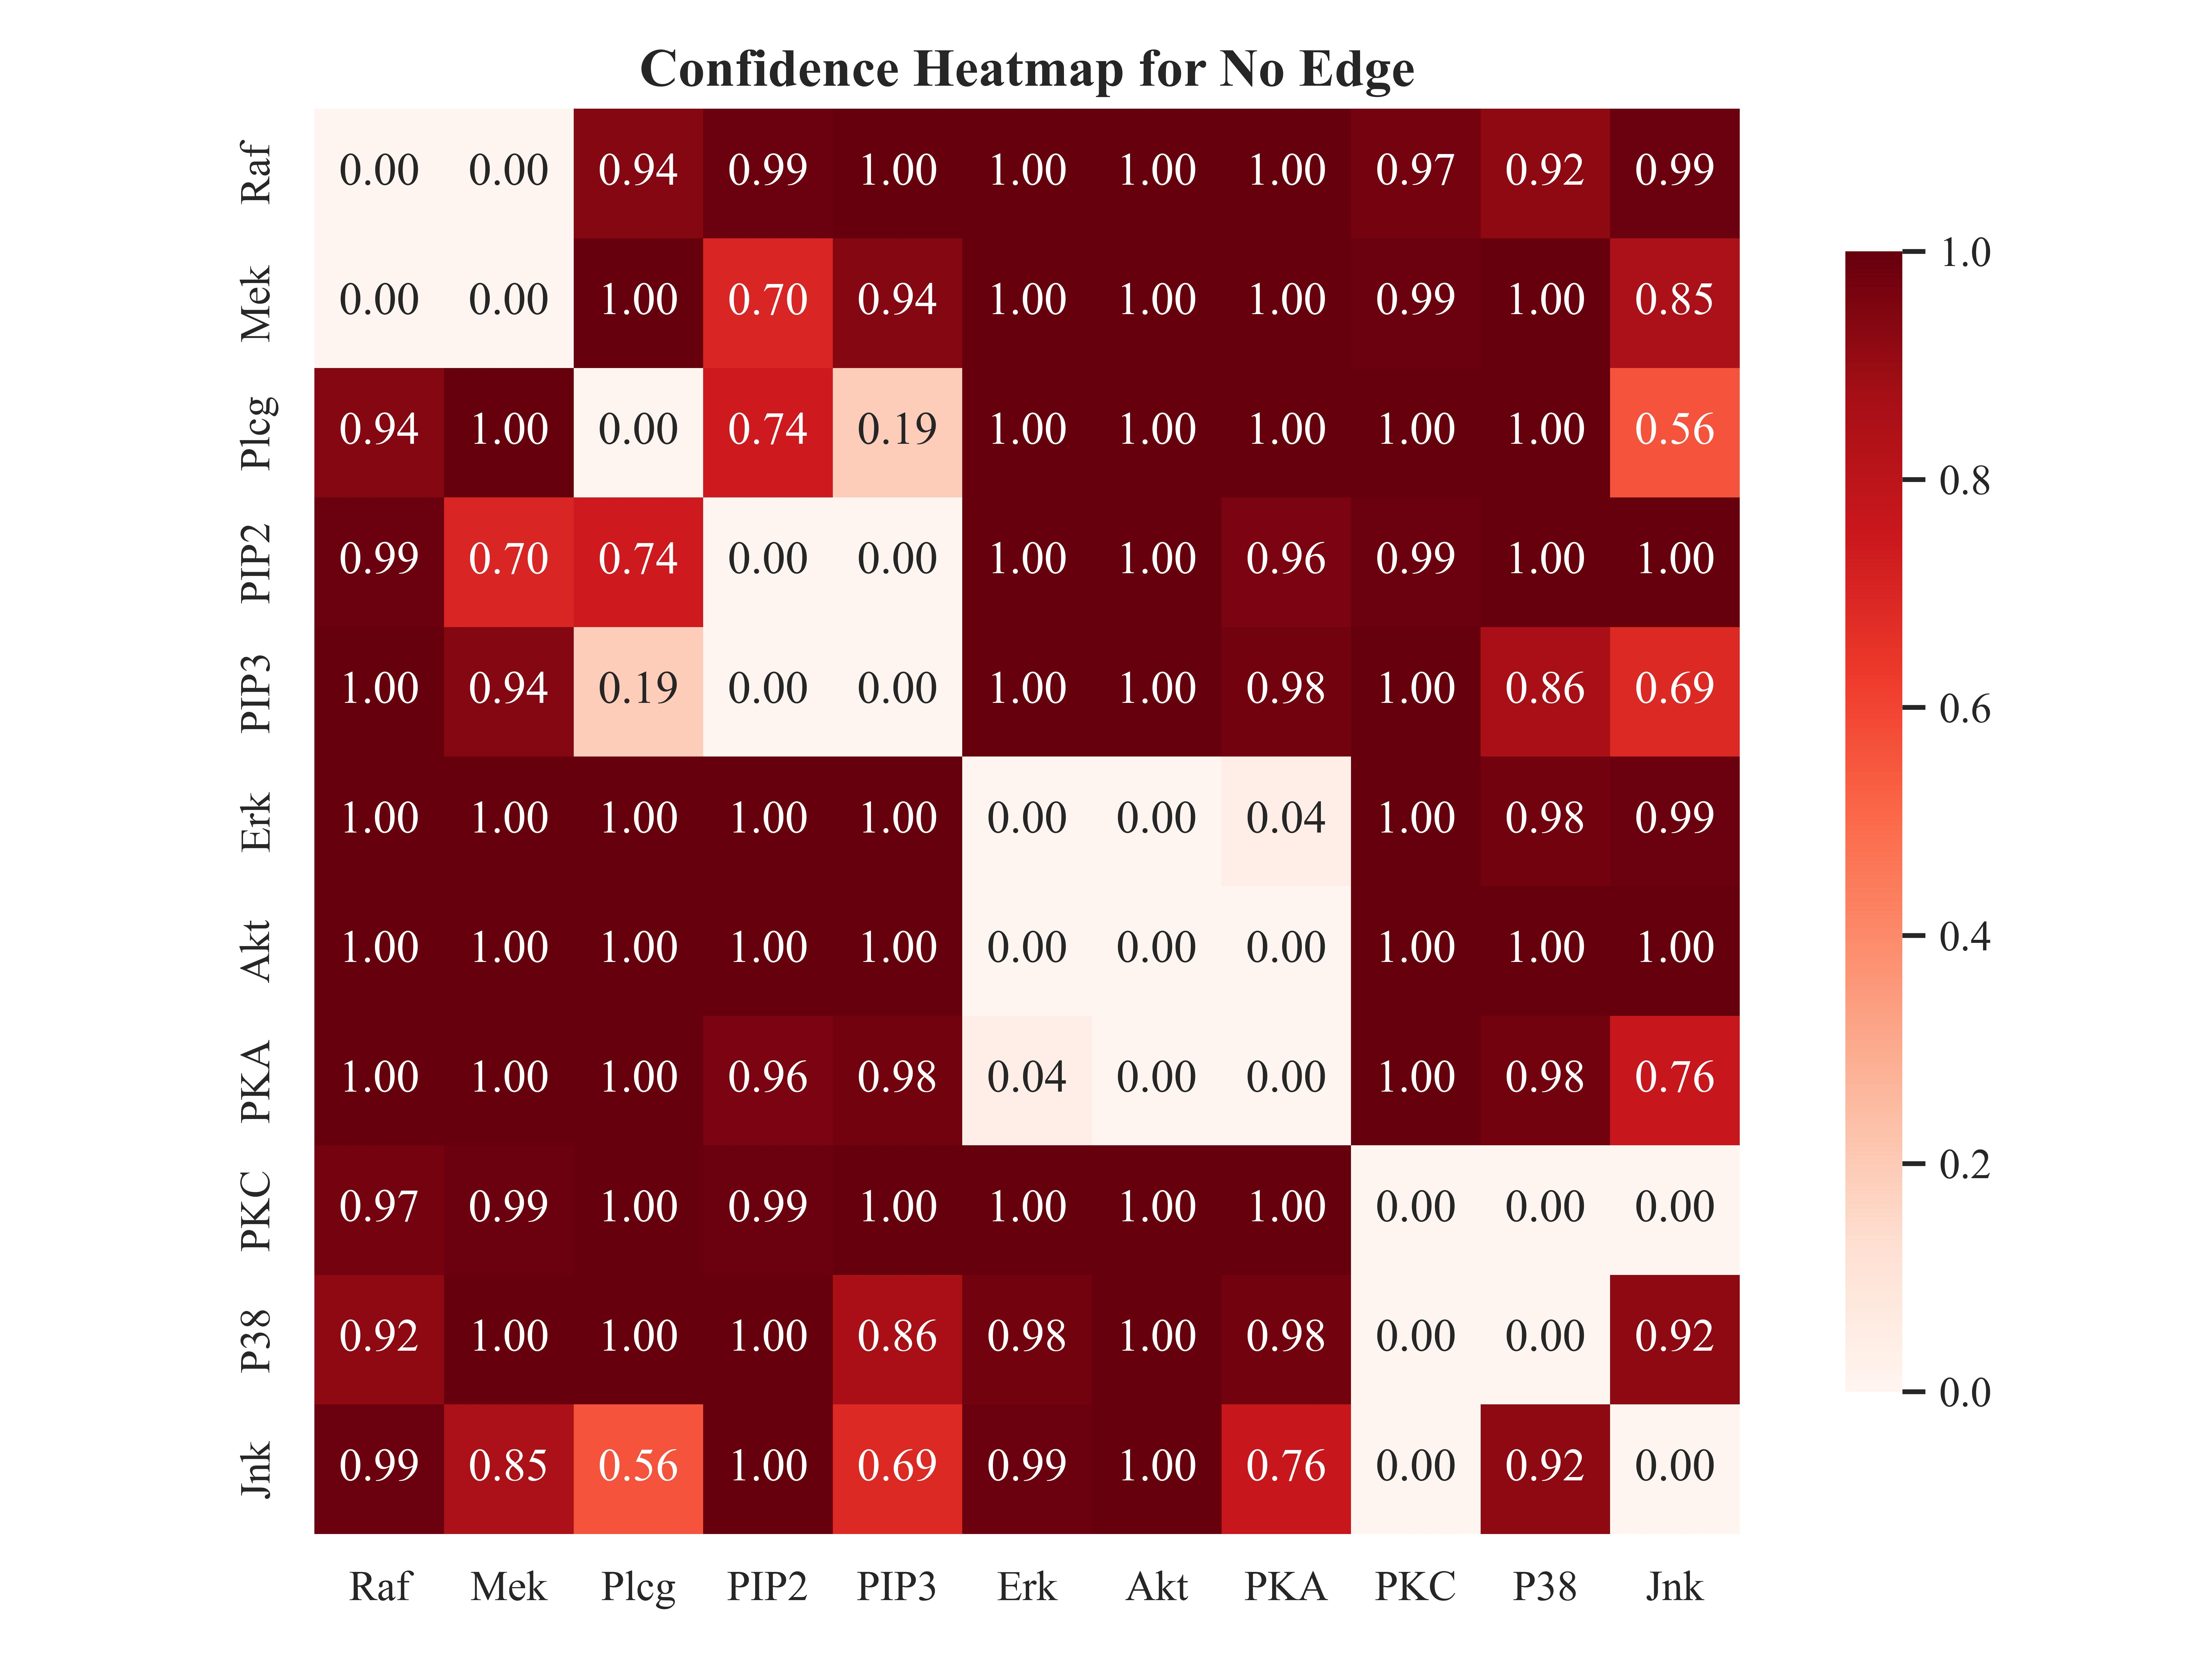
\includegraphics[width=\linewidth]{./demo_data/20241104_135804/sachs/output_graph/non_existence_confidence_heatmap.jpg}
        \caption{No Edge Edge}
\end{subfigure}
\caption{Confidence Heatmap of Different Edges}
\end{figure}        
The above heatmaps show the confidence probability we have on different kinds of edges, including directed edge ($\rightarrow$), undirected edge ($\leftrightarrow$), no edge, and probability of no edge. The heatmap of bi-edges is not shown because probabilities of all edges are 0. Based on the confidence probability heatmap and background knowledge, we can analyze the reliability of our graph.

From the statistics perspective, we have high confidence to believe that these edges exist: PIP3 $\rightarrow$ PIP2 (bootstrap probability of 0.51), PIP3 $\rightarrow$ Plcg (bootstrap probability of 0.38), and PKA $\rightarrow$ Akt (bootstrap probability of 0.21), as their probabilities indicate stronger support for causal relationships. Conversely, these edges don't exist according to our confidence levels: Raf $\rightarrow$ Mek (0.09), Erk $\rightarrow$ Akt (0.0), and P38 $\rightarrow$ PKC (0.0), showing very low confidence.

However, based on expert knowledge, we know that these edges exist: Raf $\rightarrow$ Mek (consistent with known activation pathways), Mek $\rightarrow$ Erk (a critical step in the MAPK signaling cascade), and PIP2 $\rightarrow$ PIP3 (PIP2 is a precursor for PIP3 generation). Additionally, the edges Erk $\rightarrow$ PKA and Akt $\rightarrow$ PKA may also hold relevance, even though their bootstrap scores are low. On the other hand, we can assert that edges like Akt $\rightarrow$ Erk and Akt $\rightarrow$ PKA are not established based on biological significance, as Akt primarily functions downstream in the signaling cascade.

Therefore, the result of this causal graph is partially reliable, particularly for edges with a solid grounding in expert knowledge, such as Raf $\rightarrow$ Mek and Mek $\rightarrow$ Erk. Nonetheless, edges with low bootstrap probabilities and those not supported by biological pathways indicate the need for further validation and possibly caution in interpreting these relationships.

\end{document}